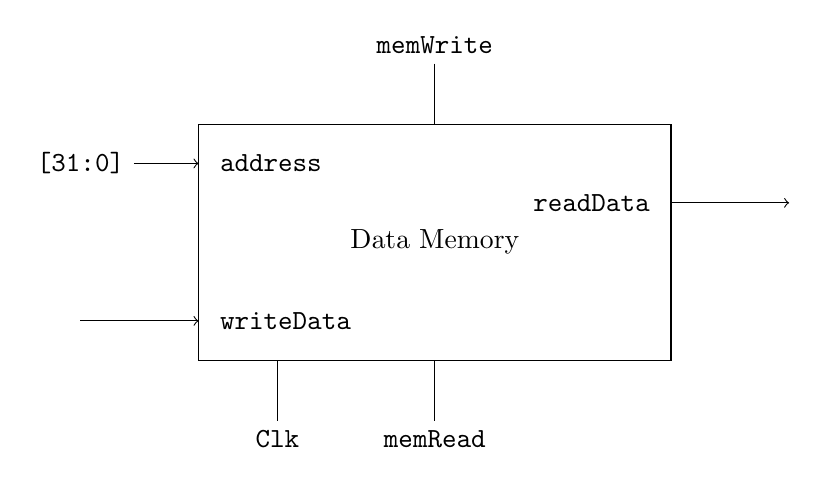
\begin{tikzpicture}
\tikzstyle{io}=[font=\ttfamily];
\tikzstyle{lio}=[io,right,xshift=-1em];
\tikzstyle{rio}=[io,left,xshift=1em];

\draw  (-1.5,2) rectangle (4.5,-1);
\node[lio] at (-1,1.5) {address};
\node[lio] at (-1,-0.5) {writeData};
\node[io] (v2) at (1.5,-2) {memRead};
\node[rio] at (4,1) {readData};
\node[io] (v1) at (-0.5,-2) {Clk};
\draw (v1) -- (-0.5,-1);
\draw (v2) -- (1.5,-1);

\draw (-3,1.5) node [io] {[31:0]} edge[->] (-1.5,1.5);
\draw (-3,-0.5) edge[->] (-1.5,-0.5);
\draw (4.5,1) edge[->] (6,1);
\node at (1.5,0.5) {Data Memory};
\node[io] (v3) at (1.5,3) {memWrite};
\draw (v3) -- (1.5,2);
\end{tikzpicture}